\documentclass[11pt,a4paper]{article}

%used packages
\usepackage{graphicx}
\usepackage[dutch]{babel} 
\usepackage{scrextend}
\usepackage{enumitem}
\usepackage{listings}
\usepackage{float}
\usepackage{titlesec}
\usepackage[table,xcdraw]{xcolor}
\usepackage{fancyhdr}
\usepackage{lastpage}
\usepackage{xcolor}
\usepackage{listings}
\usepackage{hyperref}


%Document settings
\raggedbottom
\graphicspath{ {images/} }
\setlength{\parindent}{0em}
\setlength{\parskip}{1em}

%Custom commando's
\newcommand\litem[1]{\item{\bfseries#1.\space}}
\newcommand\tabelkleur{\rowcolor[HTML]{FFCC67}}


%Custum Variables
\def\auteureen{Roy Buitenhuis, 0895833}
\def\auteurtwee{Tim van Broekhoven, 0893122}
\def\titel{Verslag TDS01} 
\def\datum{\today}
\def\versie{0.1}
\def\status{concept}
\def\subtitel{Plan van aanpak}
\def\bedrijf{}
\def\tabelkleur{FFCC67}

%Settings for Footer and Header
\pagestyle{fancy}
\fancyhf{}
\rhead{\subtitel}
\lhead{\titel}
\lfoot{\datum}
\rfoot{Pagina \thepage \hspace{1pt} /  \pageref{LastPage}}

%Settings for document spacing
\titlespacing{\section}{0pt}{*0}{*0}
\titlespacing{\subsection}{0pt}{*0}{*0}
\titlespacing{\subsubsection}{0pt}{*0}{*0}

%Settings for code sinppeds
\lstset{basicstyle=\ttfamily,
	showstringspaces=false,
	commentstyle=\color{red},
	keywordstyle=\color{blue},
	columns=fullflexible,
	frame=single,
	breaklines=true,
	postbreak=\mbox{\textcolor{red}{$\hookrightarrow$}\space},
}

\begin{document}
	
	\begin{titlepage}
		
		\centering
		{\huge\bfseries \titel \par}
		
		\vspace{1cm}
		{\Large\itshape \auteureen \par}
		{\Large\itshape \auteurtwee \par}
		\vspace{1cm}
		{\Large\itshape versie \versie\par}
				
		\vfill
		Vak:\par
		TDS01
		
		\vfill
		{\large \datum \par}
	\end{titlepage}

	\section{Samenvatting}
	
	\clearpage
	
	\tableofcontents
	
	\clearpage
	
	\listoffigures
	
	\clearpage
	\listoftables
	
	\clearpage
	
	\section{Versiehistorie}
	\begin{table}[H]
		\centering
		\label{Versiehistorie}
		\begin{tabular}{|p{1cm}|p{2cm}|p{6cm}|p{2cm}|}
			\hline
			\rowcolor[HTML]{FFCC67}
			\textbf{Versie} & \textbf{Datum} & \textbf{Wijzigingen} & \textbf{Auteur} \\ \hline
			0.1    & 25-10-2017 & Template    & Tim \\ \hline
			0.2	   & 31-10-2017 & Oplevering eerste versie  & Groep \\ \hline
			&       &             &        \\ \hline
		\end{tabular}
		\caption {Versiehistorie} \label{tab:title} 
	\end{table}	


	\section{Introductie}
		\subsection{Het vak}
		TDS02 is een van de vakken die tijdens de minor 'Embedded Systems' wordt gegeven. Het vak bestaat voornamelijk uit practicum assignments die de studenten in groepjes van twee dienen te voltooien. In de eerste weken begint de les met een uitleg van de docent over de theorie achter deze assignments, die het doel hebben om de studenten te trainen in digitale signaalbewerking. Om de assignments te voltooien dienen de studenten gebruik te maken van de 'C5505 eZdsp Development Tool' van Texas Instruments.
		
		\subsection{Introductie DSP}
		Volgens Analog Devices \cite{analog} is een DSP een processor die een  	gedigitaliseerd signaal als geluid, video, temperatuur of positie op wiskundige wijze manipuleerd. Analog Devices ligt toe dat een DSP wordt ontworpen om berekeningen als "optellen", "aftrekken", "vermenigvuldigen" en "delen" in korte tijd te kunnen voltooien. Het doel van deze berekeningen is om met de informatie van het ingangssignaal een uitgangssignaal te produceren die bruikbaar is voor een bepaalde toepassing. 
		
		\subsection{Digitale filter}
		Een digitale filter bewerktt een digitaal en tijd-discrete signaal om bepaalde frequenties uit dat signaal te verwijderen.
		
		Bron: http://www.dspguide.com/ch14/1.htm
		boek ook in pdf  			
		
		\subsection{De opdracht}		
		
				
	
	\section{Ontwerp en realisatie FIR filter}
	
	\subsection{What where the requirements for this filter?}
	Het filter dat ons groepje heeft moeten implementeren was een hoogdoorlaatfilter met een cut-off frequentie van 1500 hertz. 
	Het filter moet een minimale orde van 20 hebben. Er moest gebruik worden gemaakt van het blackmann-window.
	
	\subsection{How are the coefficients determined?}
	Als samplerate is gekozen voor 8000 hertz. Dit is genoeg om de werking van het filter te kunnen aantonen, maar maakt het filter ongeschikt voor toepassingen in geluid. 
	Kwa orde is gekozen voor een 100'ste orde filter. Dit hebben we gedaan om de lijn van het filter stijler te maken.
	Het filter is gequantificeerd voor fixed-point getallen. Dit omdat de EzDSP beter presteerd met fixed-point getallen.

	
		\begin{enumerate}[label=\emph{\alph*)}]
			\litem{item} Describe the settings you 					used in MATLAB’s FDAtool and explain the 					choices you made.
		\end{enumerate}
	

		\subsection{Matlab}
		
		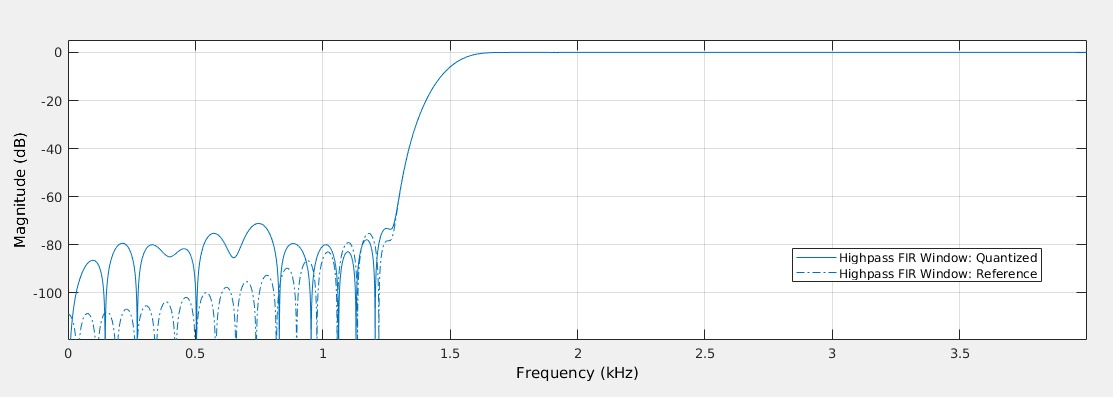
\includegraphics[width=0.80\textwidth]{firMatlab}\par\vspace{1cm}
		
		\subsection{Code}

		\begin{lstlisting}
			%code
		\end{lstlisting}
		
		\subsection{Het resultaat}

	
	\section{Ontwerp en realisatie IIR filter}
		
		\subsection{Requirements IIR filter}
	
		\subsection{Coefficienten bepalen}
	
		\begin{enumerate}[label=\emph{\alph*)}]
			\litem{item} Describe the settings you 					used in MATLAB’s FDAtool and explain the 					choices you made.
		\end{enumerate}
	
		\subsection{Matlab}
	
		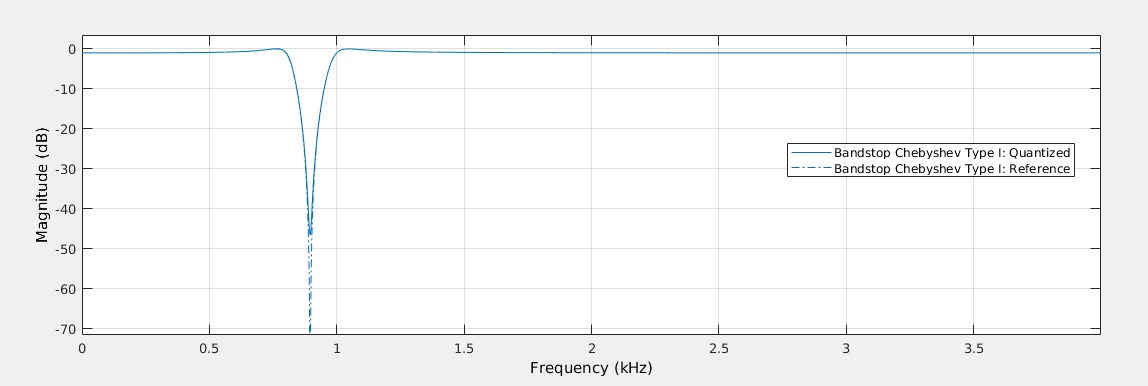
\includegraphics[width=0.80\textwidth]{iirMatlab}\par\vspace{1cm}		
		
		\subsection{Code}

		\begin{lstlisting}
			%code
		\end{lstlisting}
		
		\subsection{Het resultaat}	

	\subsection{Show charts and tables of your filter design generated by MATLAB.}
	\clearpage
	
	\subsection{De (ongeoptimalizeerde) code}
	\subsubsection{de main code.}

	\begin{lstlisting}[language=c]
#include <stdio.h>
#include <usbstk5505.h>
#include <usbstk5505_led.h>
#include <csl_intc.h>

#include "aic3204.h"
#include "fdacoefs.h"
#include "fir_buffer.h"

#define SAMPLES_PER_SECOND 8000 // possible values: 48000, 24000, 16000, 12000, 9600, and 8000
#define ADC_GAIN  0// range: 0dB to 48 dB
#define DAC_GAIN 0// range: -6dB to 29dB


extern void VECSTART(void);

FIRBuffer *buffer;
interrupt void I2S0receive() {

    fir_buffer_store_sample(buffer, AIC3204_readLeft());
    AIC3204_writeLeft(fir_buffer_output_sample(buffer, COEFFICIENTS));

}

int main(void) {
    buffer = fir_buffer_new(COEFFICIENTS_LENGTH);

    USBSTK5505_init();
    AIC3204_init(SAMPLES_PER_SECOND, ADC_GAIN, DAC_GAIN);
    IRQ_setVecs((Uint32)(&VECSTART));
    IRQ_plug(PROG1_EVENT,&I2S0receive);
    IRQ_enable(PROG1_EVENT);
    IRQ_globalEnable();

    while(1);
}
	\end{lstlisting}
	\clearpage	

	\subsubsection{De header van de fir buffer}
	\begin{lstlisting}[language=c]
#ifndef __FIR_BUFFER__
#define __FIR_BUFFER__

#include <csl_intc.h>

typedef struct {
    int size;
    Int16 *buffer;
    int currentBufferIndex;
} FIRBuffer;

FIRBuffer * fir_buffer_new(int size);
void fir_buffer_store_sample(FIRBuffer *buffer, Int16 sample);
Int16 fir_buffer_output_sample(FIRBuffer *buffer, const Int16 *coefficients);

#endif//__FIR_BUFFER__

	\end{lstlisting}
	\clearpage

	\subsubsection{Code van de fir buffer}
	\begin{lstlisting}[language=c]
#include <stdlib.h>
#include "fir_buffer.h";

FIRBuffer * fir_buffer_new(int size) {
   FIRBuffer *firBuffer = (FIRBuffer *)malloc(sizeof(FIRBuffer));
   //TODO: Still have to solve potential nullpointer issues.

   firBuffer->size = size;
   firBuffer->buffer = malloc(sizeof(Int16) * size);
   firBuffer->currentBufferIndex = 0;

   return firBuffer;
}

void fir_buffer_store_sample(FIRBuffer *buffer, Int16 sample) {
    buffer->currentBufferIndex += 1;

    if(buffer->currentBufferIndex == buffer->size) {
            buffer->currentBufferIndex = 0;
    }

    buffer->buffer[buffer->currentBufferIndex] = sample;
}

Int16 fir_buffer_output_sample(FIRBuffer *buffer, const Int16 *coefficients) {
    Int32 output = 0;
    int k;
    for(k = 0; k < buffer->size; k++){
        int bufferIndex = buffer->currentBufferIndex - k;
        if(bufferIndex < 0){
            bufferIndex += buffer->size;
        }
        output += (Int32)coefficients[k] * (Int32)buffer->buffer[bufferIndex];
    }

    return((Int16)(output >> 15));
}
	\end{lstlisting}
	\clearpage	

	\begin{lstlisting}[language=c]
/*
* Filter Coefficients (C Source) generated by the Filter Design and Analysis Tool
* Generated by MATLAB(R) 9.2 and the DSP System Toolbox 9.4.
* Generated on: 09-Oct-2017 11:48:44
*/

/*
* Discrete-Time FIR Filter (real)
* -------------------------------
* Filter Structure  : Direct-Form FIR
* Filter Length     : 101
* Stable            : Yes
* Linear Phase      : Yes (Type 1)
* Arithmetic        : single
*/
/*
* Warning - Filter coefficients were truncated to fit specified data type.  
*   The resulting response may not match generated theoretical response.
*   Use the Filter Design & Analysis Tool to design accurate
*   int16 filter coefficients.
*/
#include <csl_intc.h>
#define COEFFICIENTS_LENGTH 101

const Int16 COEFFICIENTS[COEFFICIENTS_LENGTH] = {
0,      0,      0,      1,      1,     -1,     -3,     -2,      4,
7,      0,    -12,    -12,      8,     25,     12,    -26,    -40,
0,     55,     49,    -31,    -94,    -41,     88,    131,      0,
-170,   -147,     90,    266,    115,   -238,   -350,      0,    443,
381,   -233,   -686,   -298,    626,    938,      0,  -1271,  -1159,
767,   2541,   1311,  -3664,  -9621,  20480,  -9621,  -3664,   1311,
2541,    767,  -1159,  -1271,      0,    938,    626,   -298,   -686,
-233,    381,    443,      0,   -350,   -238,    115,    266,     90,
-147,   -170,      0,    131,     88,    -41,    -94,    -31,     49,
55,      0,    -40,    -26,     12,     25,      8,    -12,    -12,
0,      7,      4,     -2,     -3,     -1,      1,      1,      0,
0,      0
};	
	\end{lstlisting}
	\clearpage


	\subsection{Het resultaat}
	\clearpage
	
	\section{Ontwerp en realisatie IIR filter}
	\subsection{What where the requirements for this filter?}
	
	\subsection{How are the coefficients determined?}
	
	\begin{enumerate}[label=\emph{\alph*)}]
		\litem{item} Describe the settings you 					used in MATLAB’s FDAtool and explain the 					choices you made.
	\end{enumerate}

	\subsection{Show charts and tables of your filter design generated by MATLAB.}
	\subsection{De (ongeoptimalizeerde) code}

	\subsubsection{de main code.}
	\begin{lstlisting}[language=c]
#include <stdio.h>
#include <usbstk5505.h>
#include <usbstk5505_led.h>
#include <csl_intc.h>
#include <iir_buffer.h>

#include "aic3204.h"
#include "iir_fdacoefs3.h"

#define SAMPLES_PER_SECOND 8000 // possible values: 48000, 24000, 16000, 12000, 9600, and 8000
#define ADC_GAIN  0// range: 0dB to 48 dB
#define DAC_GAIN 0// range: -6dB to 29dB


extern void VECSTART(void);


IIRBuffer *buffer;
interrupt void I2S0receive() {
	iir_buffer_store_sample(buffer, AIC3204_readLeft());
	AIC3204_writeLeft(iir_buffer_output_sample(buffer, DEN, NUM));

}

int main(void) {
	buffer = iir_buffer_new(COEFFICIENTS_LENGTH, 1);

	USBSTK5505_init();
	AIC3204_init(SAMPLES_PER_SECOND, ADC_GAIN, DAC_GAIN);
	IRQ_setVecs((Uint32)(&VECSTART));
	IRQ_plug(PROG1_EVENT,&I2S0receive);
	IRQ_enable(PROG1_EVENT);
	IRQ_globalEnable();

	while(1);
}
	\end{lstlisting}
	\clearpage
	
	\subsubsection{IIR buffer header}
	\begin{lstlisting}[language=c]
#ifndef __IIR_BUFFER__
#define __IIR_BUFFER__

#include <csl_intc.h>

typedef struct {
	int size;
	int sections;
	Int16 *buffer;
	Int32 *outputBuffer;
	int currentBufferIndex;
} IIRBuffer;

IIRBuffer * iir_buffer_new(int size, int sections);
void iir_buffer_store_sample(IIRBuffer *buffer, Int16 sample);
Int16 iir_buffer_output_sample(IIRBuffer *buffer, const Int16 *denominator, const Int16 *numerator);

#endif//__IIR_BUFFER__
		
	\end{lstlisting}
	\clearpage
	
	\subsubsection{IIR buffer source}
	\begin{lstlisting}[language=c]
#include <iir_buffer.h>
#include <stdlib.h>

Int32 direct_form_1(IIRBuffer *buffer, Int32 input, const Int16 *denominator, const Int16 *numerator) {
	Int32 output = input;
	int k;
	for(k = 0; k < buffer->size; k++){
		int bufferIndex = buffer->currentBufferIndex - k;
		if(bufferIndex < 0){
			bufferIndex += buffer->size;
		}

		output += (Int32)numerator[k] * (Int32)buffer->buffer[bufferIndex];
	}

	int i;
	for(i = 1; i < buffer->size; i++) {
		int bufferIndex = buffer->currentBufferIndex - i;
		if(bufferIndex < 0){
			bufferIndex += buffer->size;
		}

		output -= (Int32)denominator[i] * (Int32)buffer->outputBuffer[bufferIndex];
	}
	return output;
}

IIRBuffer * iir_buffer_new(int size, int sections) {
	IIRBuffer *iirBuffer = (IIRBuffer *)malloc(sizeof(IIRBuffer));
	//TODO: Still have to solve potential nullpointer issues.

	iirBuffer->size = size;
	iirBuffer->sections = sections;
	iirBuffer->buffer = malloc(sizeof(Int16) * size);
	iirBuffer->outputBuffer = malloc(sizeof(Int32) * size);

	int i;
	for(i = 0; i < size; i++) {
		iirBuffer->buffer[i] = 0;
		iirBuffer->outputBuffer[i] = 0;
	}

	iirBuffer->currentBufferIndex = 0;

	return iirBuffer;
}

void iir_buffer_store_sample(IIRBuffer *buffer, Int16 sample) {
	buffer->currentBufferIndex += 1;

	if(buffer->currentBufferIndex == buffer->size) {
			buffer->currentBufferIndex = 0;
	}

	buffer->buffer[buffer->currentBufferIndex] = sample;
}

Int16 iir_buffer_output_sample(IIRBuffer *buffer, const Int16 *denominator, const Int16 *numerator) {
	Int32 output = 0;

	output += direct_form_1(buffer, output, denominator, numerator);

	buffer->outputBuffer[buffer->currentBufferIndex] = output >> 13;
	return((Int16)(output>>13));
}
	\end{lstlisting}
	\clearpage
	
	\subsubsection{IIR coefficients}
	\begin{lstlisting}[language=c]
/*
* Filter Coefficients (C Source) generated by the Filter Design and Analysis Tool
* Generated by MATLAB(R) 9.2 and the DSP System Toolbox 9.4.
* Generated on: 23-Oct-2017 14:07:54
*/

/*
* Discrete-Time IIR Filter (real)
* -------------------------------
* Filter Structure    : Direct-Form I
* Numerator Length    : 5
* Denominator Length  : 5
* Stable              : Yes
* Linear Phase        : No
* Arithmetic          : fixed
* Numerator           : s16,13 -> [-4 4)
* Denominator         : s16,13 -> [-4 4)
* Input               : s16,15 -> [-1 1)
* Output              : s16,15 -> [-1 1)
* Numerator Prod      : s32,28 -> [-8 8)
* Denominator Prod    : s32,28 -> [-8 8)
* Numerator Accum     : s40,28 -> [-2048 2048)
* Denominator Accum   : s40,28 -> [-2048 2048)
* Round Mode          : convergent
* Overflow Mode       : wrap
* Cast Before Sum     : true
*/

/* General type conversion for MATLAB generated C-code  */
/* 
* Expected path to tmwtypes.h 
* /usr/local/MATLAB/R2017a/extern/include/tmwtypes.h 
*/
#define COEFFICIENTS_LENGTH 5
const Int16 NUM[5] = {
	6735, -20550,  29146, -20550,   6735
};

const Int16 DEN[5] = {
	8192, -23961,  32617, -22154,   7008
};	   
	\end{lstlisting}
	\clearpage

	\section{optimizatie}
	De enige optimalitaties is uitgevoerd heeft niets te maken met de prestaties tijdens het uitvoeren op de EzDSP. Alleen is de leesbaarheid van de code verbeterd doordat de staat van de filters in een struct wordt bijgehouden. Er zijn functies beschreven die iets in de buffer op kunnen slaan of een output sample kunnen berekenen. Hierdoor is de code ook beter herbruikbaar.
	

	\section{Conclusie en aanbevelingen}
	
	\bibliographystyle{plain}
	\bibliography{bibligraphy}
		
	\begin{thebibliography}{9}

	\bibitem{analog}
  		
  		\textit{A Beginner's Guide to Digital Signal Processing (DSP)},
  		Analog Devices,
  		URL: http://www.analog.com/en/design-center/landing-pages/001/beginners-guide-to-dsp.html 

	
	\bibitem{}
  		
  		\textit{},
  		Addison Wesley, Massachusetts,
  		2nd edition,
  		1994.
  		
	\bibitem{}
  		
  		\textit{},
  		Addison Wesley, Massachusetts,
  		2nd edition,
  		1994.  		
		
	\end{thebibliography}

\end{document}